%! TeX program = lualatex
\documentclass[a4paper]{article} 

% packages
\usepackage{microtype}      % Slightly tweak font spacing for aesthetics
\usepackage[english]{babel} % Language hyphenation and typographical rules
\usepackage[final, colorlinks = true, urlcolor = black, linkcolor = black]{hyperref} 
\usepackage{changepage}     % adjust margins on the fly

\usepackage{fontspec}
\setmainfont{EB Garamond}
\setmonofont[Scale=MatchLowercase]{Deja Vu Sans Mono}

\usepackage{minted}
\usemintedstyle{algol_nu}
\usepackage{xcolor}

\usepackage{pgfplots}
\pgfplotsset{width=\textwidth,compat=1.9}

\usepackage{caption}
\newenvironment{code}{\captionsetup{type=listing}}{}
\captionsetup[listing]{skip=0pt}
\setlength{\abovecaptionskip}{5pt}
\setlength{\belowcaptionskip}{5pt}

\usepackage[yyyymmdd]{datetime}
\renewcommand{\dateseparator}{--}

\usepackage{titlesec}
% \titleformat{\section}{\LARGE\bfseries}{}{}{}[\titlerule]
% \titleformat{\subsection}{\Large\bfseries}{}{0em}{}
% \titlespacing{\subsection}{0em}{-0.7em}{0em}
%
% \titleformat{\subsubsection}{\large\bfseries}{}{0em}{$\bullet$ }
% \titlespacing{\subsubsection}{1em}{-0.7em}{0em}

% margins
\addtolength{\hoffset}{-2.25cm}
\addtolength{\textwidth}{4.5cm}
\addtolength{\voffset}{-3.25cm}
\addtolength{\textheight}{5cm}
\setlength{\parskip}{0pt}
\setlength{\parindent}{0in}
% \setcounter{secnumdepth}{0}

\begin{document}
\hrule \medskip
\begin{minipage}{0.295\textwidth} 
    \raggedright
    \footnotesize 
    \begin{tabular}{@{}l l} % Define a two-column table with left alignment
        Name: & Andrew Hayes \\
        Student ID: & 21321503 \\
    \end{tabular}
\end{minipage}
\begin{minipage}{0.4\textwidth} 
    \centering 
    \vspace{0.4em}
    \LARGE 
    \textsc{ct404} \\ 
\end{minipage}
\begin{minipage}{0.295\textwidth} 
    \raggedleft
    \footnotesize 
    \begin{tabular}{@{}l l} % Define a two-column table with left alignment
        Name: & Maxwell Maia \\
        Student ID: & 21236277 \\
    \end{tabular}
\end{minipage}
\smallskip
\hrule 
\begin{center}
    \normalsize
    Lab Assignment 1: Camera Callibration
\end{center}
\hrule

\section{\textit{P}-Matrix Estimation Using Provided Code}
\begin{figure}[H]
    \centering
    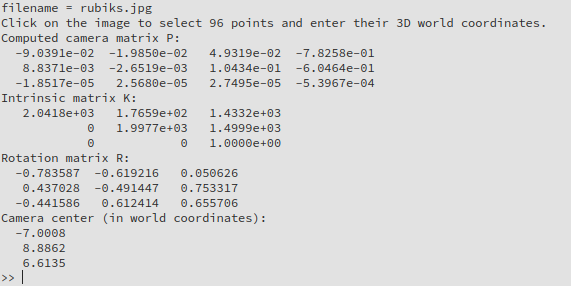
\includegraphics[width=\textwidth]{./images/1.1.png}
    \caption{ Command window output showing he computed camera matrix $P$, the intrinsic matrix $K$, \& the rotation matrix $R$ }
\end{figure}

\begin{figure}[H]
    \centering
    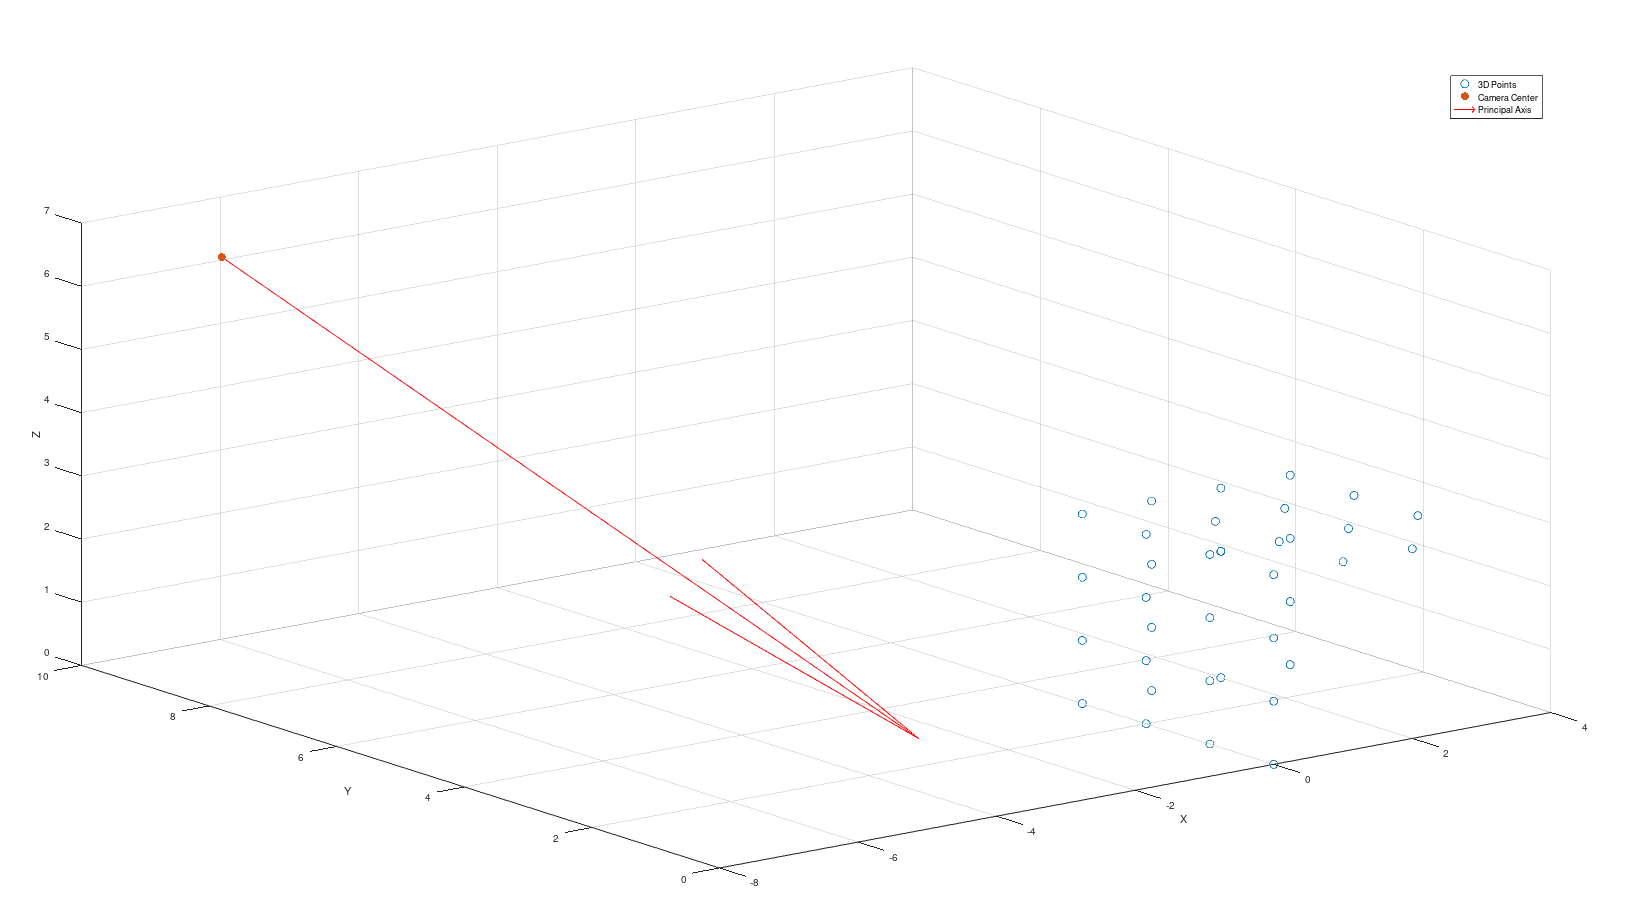
\includegraphics[width=\textwidth]{./images/1.2.png}
    \caption{ The 3D plot showing the camera center, the world points, \& the principal axis }
\end{figure}

\begin{figure}[H]
    \centering
    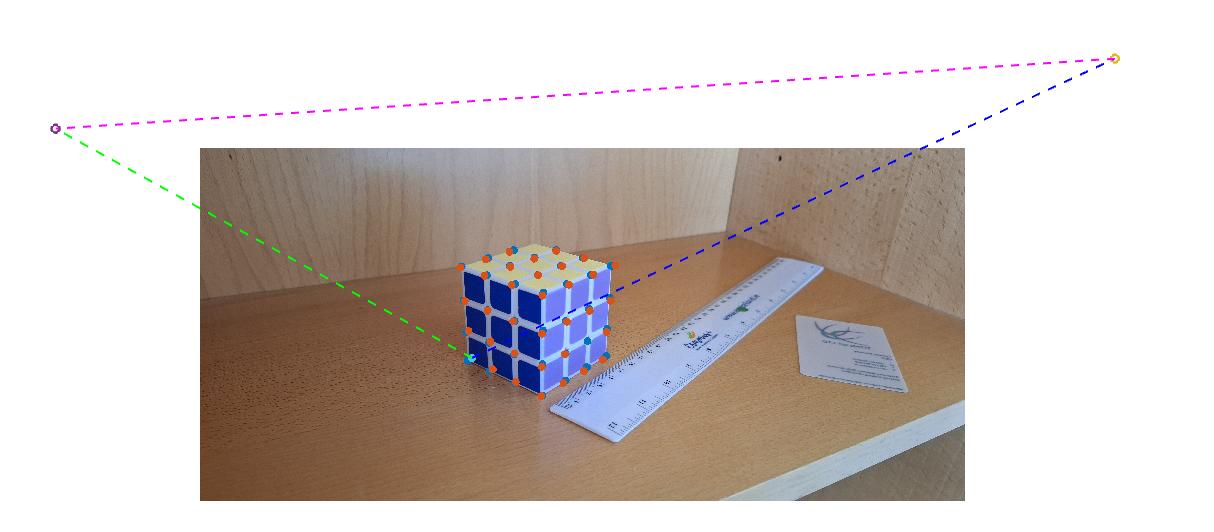
\includegraphics[width=\textwidth]{./images/1.3.png}
    \caption{ The image with projected 3D points \& vanishing lines }
\end{figure}

\section{Using Your Own Image from Your Camera for \textit{P}-Matrix Estimation}
\begin{figure}[H]
    \centering
    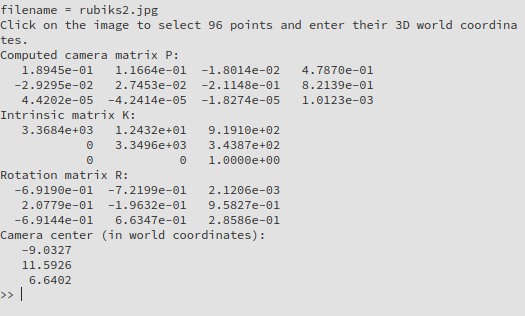
\includegraphics[width=\textwidth]{./images/2.1.png}
    \caption{ Command window output showing he computed camera matrix $P$, the intrinsic matrix $K$, \& the rotation matrix $R$ }
\end{figure}

\begin{figure}[H]
    \centering
    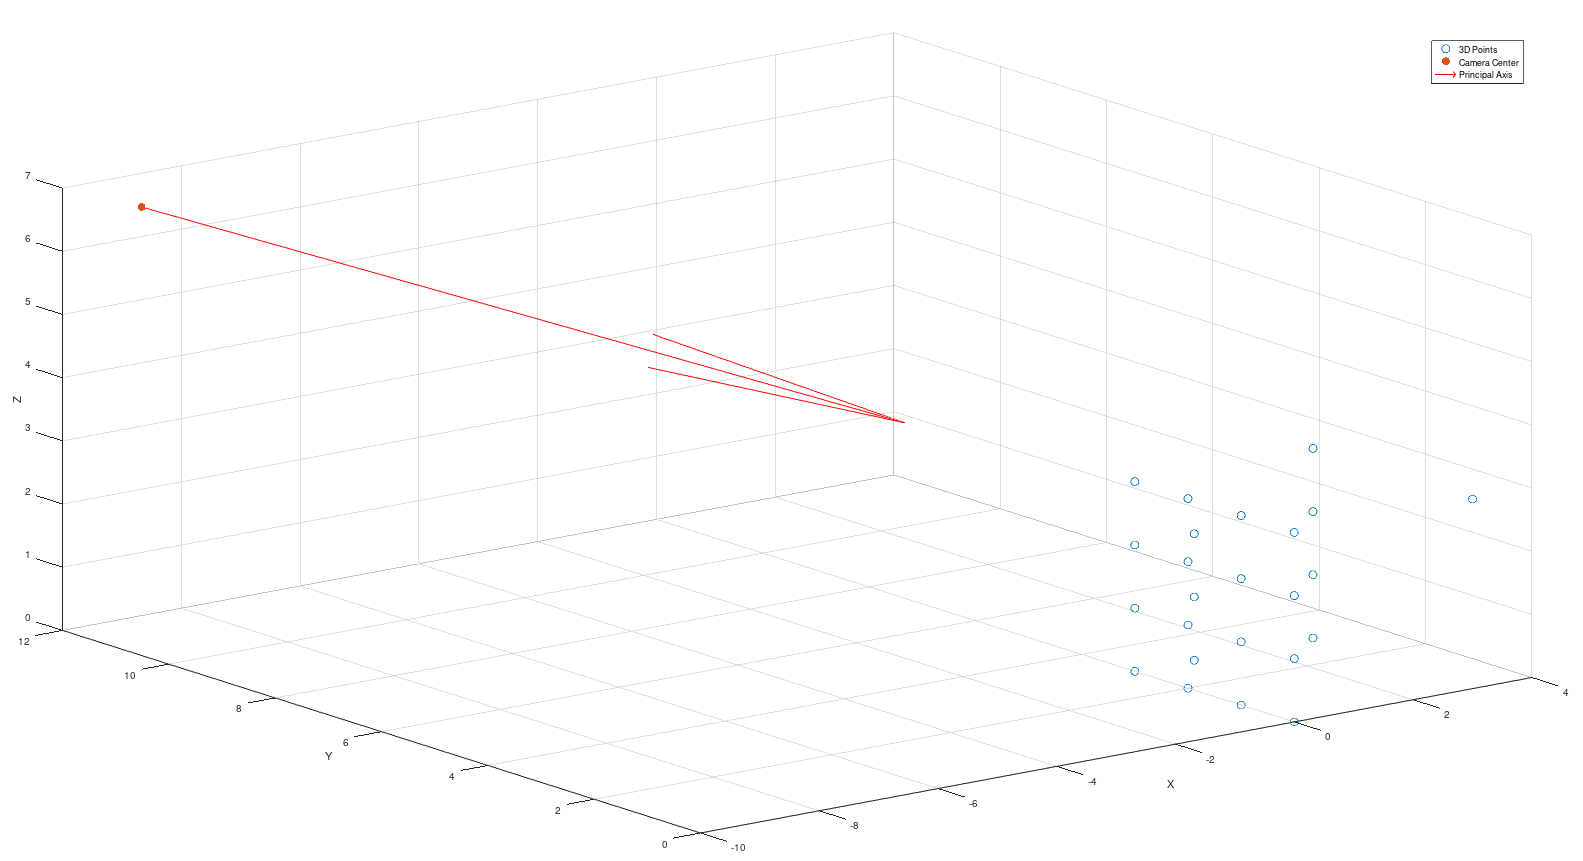
\includegraphics[width=\textwidth]{./images/2.2.png}
    \caption{ The 3D plot showing the camera center, the world points, \& the principal axis }
\end{figure}

\begin{figure}[H]
    \centering
    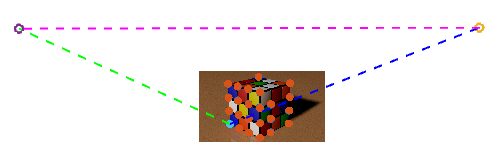
\includegraphics[width=\textwidth]{./images/2.3.png}
    \caption{ The image with projected 3D points \& vanishing lines }
\end{figure}

\section{Experiment \& Reflect}
\subsection{How does increasing the number of points affect the accuracy \& stability of the \textit{P}-matrix estimation?}
As the number of control points increased, the accuracy and stability of the estimated P Matrix improved. With 12 points, we observed discrepancies in the back-projected 3D points, while results with 40 points were far more consistent. The intrinsic and rotation matrices derived from the P Matrix appeared less sensitive to noise with more points, enhancing the reliability of the calibration.

\subsection{Is there a noticeable difference in the accuracy of the back-projection when using fewer points versus more points?}
Using fewer points (e.g., 12) resulted in higher deviations in back-projected points compared to their actual image locations. With 40 points, the back-projection closely matched the real-world setup, minimizing errors.

\subsection{What challenges did you encounter when manually selecting points \& entering 3D world coordinates?}
The primary challenge that we faced when manually entering selecting the points was the precision: it was extremely difficult to precisely select the correct points due to the imprecision of the mouse as a selection device, human error, and a lack of fine-grain zoom control in the MATLAB UI.
\\\\
We also found the process of manually entering the points very time-consuming and error-prone.
If we mis-clicked a point or accidentally entered in the wrong world coordinate, it would greatly damage the accuracy of the entire calibration and we would be forced to start over again.

\end{document}
